\subsubsection{\acrfull{ar} model}\label{model_ar}


An \acrshort{ar} model is another type of recurrent neural network. The peculiarity of this network is that the result obtained is used as an input value for the calculation of the next iteration. The graphically generated model is as follows:

\begin{figure}[H]
    \centering
    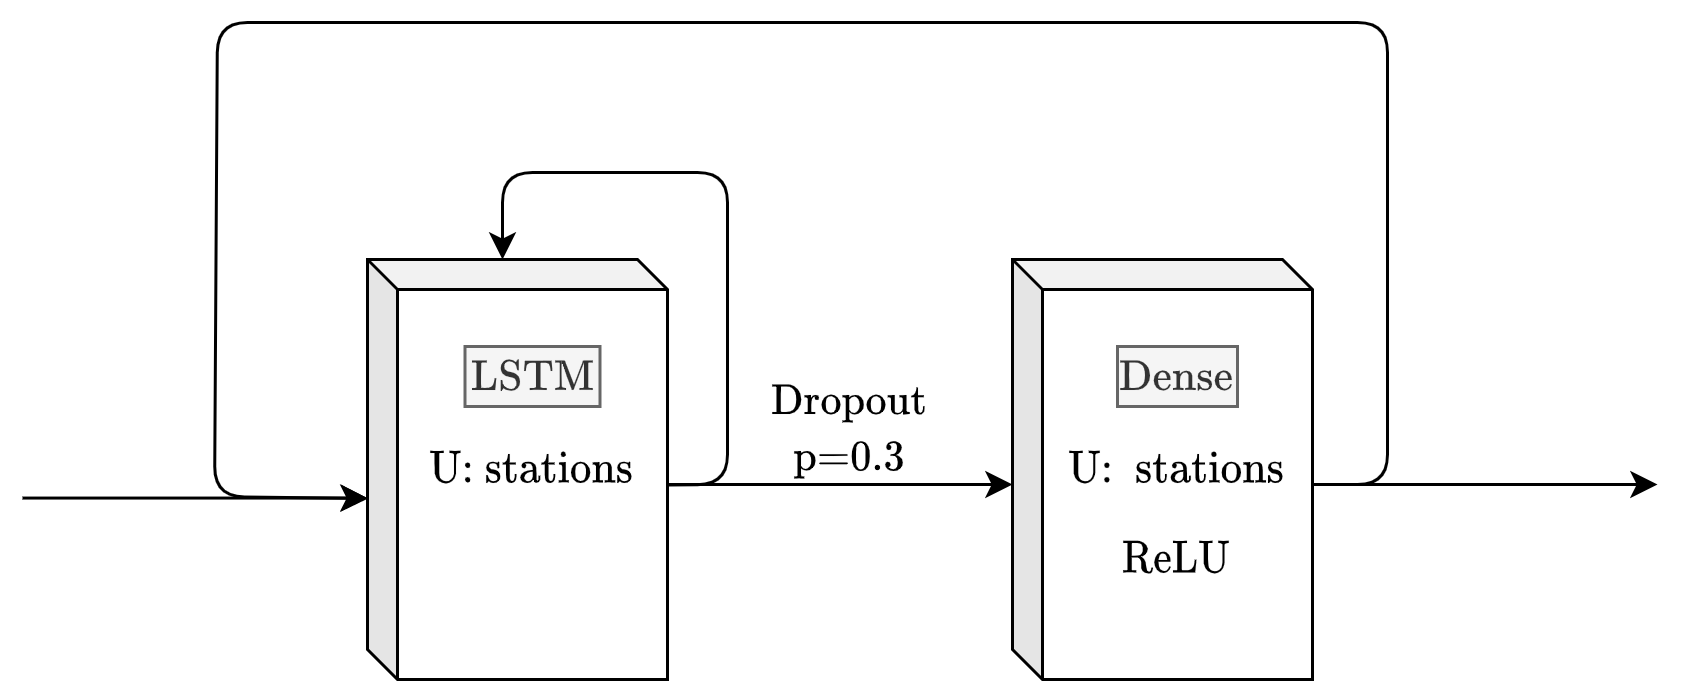
\includegraphics[width=10cm]{images/solution/models/AR.png}
    \caption{Recurrent \acrshort{ar} model}
    \label{fig:dense-model}
\end{figure}

The model has an \acrshort{lstm} layer along with a dense layer. The output of this layer which is the prediction of the model is reintroduced into the model to predict the rest of the predictions.
\newline

Tensorflow does not have a model in its tool library that meets the needs that were being sought and for that reason, this model has had to be implemented using another technique. A new class has been created that inherits from \small{\verb|tf.keras.Model|} \normalsize  and which has three methods: \small{\verb|__init__|} \normalsize , \small{\verb|warmup|} \normalsize  and \small{\verb|call|} \normalsize . In this way it is possible to generate models that can have unique architectures different from the pass-forward ones. For the implementation, the documentation of Tensorflow \cite{tensorflow2015-whitepaper} and Keras \cite{keras} has been followed. The code developed for this class can be read in Appendix \ref{app:ar}.
\newline

To create a new \acrshort{ar} model simply generate a new instance as follows:

\begin{minted}[fontsize=\scriptsize]{python}
AutoRegressive(lstm_units=stations, steps=steps, stations=stations)
\end{minted}

The results of the model can be seen together with the other results in section \ref{results}.